%%%%%%%%%%%%%%%%%%%%%%%%%%%%%%%%%%%%%%%%%%%%%%%%%%%
%
%  New template code for TAMU Theses and Dissertations starting Fall 2012.  
%  For more info about this template or the 
%  TAMU LaTeX User's Group, see http://www.howdy.me/.
%
%  Author: Wendy Lynn Turner 
%	 Version 1.0 
%  Last updated 8/5/2012
%
%%%%%%%%%%%%%%%%%%%%%%%%%%%%%%%%%%%%%%%%%%%%%%%%%%%

%%%%%%%%%%%%%%%%%%%%%%%%%%%%%%%%%%%%%%%%%%%%%%%%%%%%%%%%%%%%%%%%%%%%%%
%%                           SECTION 4
%%%%%%%%%%%%%%%%%%%%%%%%%%%%%%%%%%%%%%%%%%%%%%%%%%%%%%%%%%%%%%%%%%%%%%

%%%%%%%%%%%%%%%%%%%%%%%%%%%%%%%%%%%%%%%%%%%%%%%%%%%%%%%%%%%%%%%%%%%%%%
\chapter{\uppercase {Application of the entropy viscosity method to the seven equations model.}}\label{chap:seven}
%%%%%%%%%%%%%%%%%%%%%%%%%%%%%%%%%%%%%%%%%%%%%%%%%%%%%%%%%%%%%%%%%%%%%%
%===================================================================================
\section{Description of the seven equation model:}
%===================================================================================
Because it is not economical to solve the entire two-phase flow field
with highly resolved three-dimensional computational fluid dynamics for an
entire light water reactor coolant system,
it is necessary to construct a one-dimensional model for flow in
pipes, nozzles, and other components.  The one-dimensional model is
constructed to allow the representation of continuously variable
cross-sectional area.

Consider flow through a duct with local cross-sectional area
$A=A(x,t)$.  Actually, most of the time we consider local
cross-sectional area to depend upon position coordinate $x$ only,
for which a time rate of change of cross-sectional area is not
necessary because for this case $\frac{\partial A}{\partial
t} = 0$.  However, $A(x,t)$ is left inside the time derivative terms
for generality and possible future use.  The seven-equation two-phase
system model can be stated as balances of mass, momentum, and total energy,
along with volume fraction evolution as
\begin{align}
  % liquid mass conservation
  \label{E-R:74}
  \frac{\partial \left( \alpha \rho \right)_{liq} A}{\partial t}
  + \frac{\partial \left( \alpha \rho u \right)_{liq} A}{\partial x}
  &= - \Gamma A_{int} A
  \\
  % liquid momentum
  \nonumber
  \frac{\partial \left( \alpha \rho u \right)_{liq} A}{\partial t}
  + \frac{\partial \alpha_{liq} A \left( \rho u^2 + p \right)_{liq} }{\partial x}
  &= p_{int} A \frac{\partial \alpha_{liq}}{\partial x} + p_{liq} \alpha_{liq} \frac{\partial A}{\partial x}
  \\
  \nonumber
  &+ A \lambda (u_{vap} - u_{liq})
  \\
  \nonumber
  &- \Gamma A_{int} u_{int} A
  \\
  \nonumber
  &- F_{\text{wall friction}, liq} - F_{\text{friction}, vap}
  \\
  &+ \left( \alpha \rho \right)_{liq} A \vec{g} \cdot \vec{n}_{axis}
\end{align}
\begin{align}
  % liquid total energy
  \nonumber
  \frac{\partial \left( \alpha \rho E \right)_{liq} A}{\partial t}
  + \frac{\partial \alpha_{liq} u_{liq} A \left( \rho E + p \right)_{liq}}{\partial x}
  &= p_{int} u_{int} A \frac{\partial \alpha_{liq}}{\partial x} - \bar{p}_{int} A \mu (p_{liq} - p_{vap})
  \\
  \nonumber
  &+ \bar{u}_{int} A \lambda (u_{vap} - u_{liq})
  \\
  \nonumber
  &+ \Gamma A_{int} \left( \frac{p_{int}}{\rho_{int}} - H_{liq, int} \right) A
  \\
  &+ Q_{int, liq} + Q_{\text{wall}, liq}
  \\
  % liquid volume fraction
  \label{eqn:7eqn_va_alpha_liq}
  \frac{\partial \alpha_{liq} A}{\partial t} + u_{int} A \frac{\partial \alpha_{liq}}{\partial x}
  &= A \mu (p_{liq} - p_{vap}) - \frac{\Gamma A_{int} A}{\rho_{int}}
\end{align}
for the liquid phase, and
\begin{align}
  % vapor mass conservation
  \frac{\partial \left( \alpha \rho \right)_{vap} A}{\partial t}
  + \frac{\partial \left( \alpha \rho u \right)_{vap} A}{\partial x}
  &=  \Gamma A_{int} A
  \\
  % vapor momentum
  \nonumber
  \frac{\partial \left( \alpha \rho u \right)_{vap} A}{\partial t}
  + \frac{\partial \alpha_{vap} A \left( \rho u^2 + p \right)_{vap} }{\partial x}
  &= p_{int} A \frac{\partial \alpha_{vap}}{\partial x} + p_{vap} \alpha_{vap} \frac{\partial A}{\partial x}
  \\
  \nonumber
  &+ A \lambda (u_{liq} - u_{vap})
  \\
  \nonumber
  &+ \Gamma A_{int} u_{int} A
  \\
  \nonumber
  &- F_{\text{wall friction}, vap} - F_{\text{friction}, liq}
  \\
  &+ \left( \alpha \rho \right)_{vap} A \vec{g} \cdot \vec{n}_{axis}
\end{align}
\begin{align}
  \nonumber
  % vapor total energy
  \frac{\partial \left( \alpha \rho E \right)_{vap} A}{\partial t}
  + \frac{\partial \alpha_{vap} u_{vap} A \left( \rho E + p \right)_{vap}}{\partial x}
  &= p_{int} u_{int} A \frac{\partial \alpha_{vap}}{\partial x} - \bar{p}_{int} A \mu (p_{vap} - p_{liq})
  \\
  \nonumber
  &+ \bar{u}_{int} A \lambda (u_{liq} - u_{vap})
  \\
  \nonumber
  &- \Gamma A_{int} \left( \frac{p_{int}}{\rho_{int}} - H_{vap, int} \right) A
  \\
  &+ Q_{int, vap} + Q_{\text{wall}, vap}
  \\
  % vapor phase volume fraction
  \label{E-R:81}
  \frac{\partial \alpha_{vap} A}{\partial t} + u_{int} A \frac{\partial \alpha_{vap}}{\partial x}
  &= A \mu (p_{vap} - p_{liq}) + \frac{\Gamma A_{int} A}{\rho_{int}}
\end{align}
for the vapor phase.  It is noted that for two-phase flow,
either of the differential relations~\eqref{eqn:7eqn_va_alpha_liq}
or~\eqref{E-R:81} may be replaced with the algebraic relation
\begin{align}
 \alpha_{vap}= 1 - \alpha_{liq}
\end{align}
throughout, reducing the total number of equations to be solved to seven.

In equations~\eqref{E-R:74}--\eqref{E-R:81}, $\Gamma$ is the net mass transfer per unit
interfacial area from the liquid to the vapor phase and $A_{int}$ is
the interfacial area per unit volume of mixture.  Also, $H_{liq, int}$
and $H_{vap, int}$ are the liquid and gas total enthalpies at the
interface, respectively.  The nomenclature has also been modified so
that now $u_{int}$ and $\bar{u}_{int}$ are, respectively, the
interfacial velocity and average interfacial velocity; and $p_{int}$
and $\bar{p}_{int}$ are, respectively, the interfacial pressure and
average interfacial pressure.  In the momentum balance equations
$\vec{n}_{axis}$ is the unit vector directly along the axis of the
duct, which is also the $\pm$ flow direction.  Of course
$F_{\text{wall friction}, k}$ is the frictional force due to the wall acting on phase
$k$ and $F_{\text{friction}, k'}$ is the frictional force acting on
phase $k$ due to the presence of the other phase $k'$.
Similarly, $Q_{int, k}$ is the direct heat transfer from the interface
to phase $k$ and $Q_{\text{wall}, k}$ is the direct heat transfer from
the wall to phase $k$.

Equation system~\eqref{E-R:74}--\eqref{E-R:81} is the basic system
solved with RELAP-7.  The system was implemented within the MOOSE
computational framework following a series of logically-complete
steps~\cite{Berry_2013} designed to confidently allow physically- and
mathematically-meaningful benchmark testing at each step of increased
complexity.  This 7-equation two-phase model allows both phases to be
compressible.

\subsection{Seven-Equation Two-Phase Flow Constitutive Models}
Without additional closure equations the balance relations derived
above are generic, i.e.\ they apply to all materials (fluids).  They
must made to apply to the unique material (fluid) being considered --
material specific.  Also, though averaging the microlevel
balance equations led to the ``simplified'' or perhaps more tractable
model above, this simplification (averaging) led to a loss of information,
and some additional relations must also be specified to supply (or
restore) at least some information that was lost in this
process\footnote{The process of averaging the balance equations produced a
system with more unknowns than equations; thus postulates or empirical
correlations are required to resolve this deficiency.}.  Collectively,
any additional relations, or sub-models, that must be specified to
render mathematical closure (allowing a solution to be obtainable) to
the generic balance equations are known as ``constitutive
relations''.

Because the 7-equation two-phase model's most unique features are
reflected in the presence of a volume fraction evolution equation,
interfacial pressure and velocity, and mechanical relaxation terms
involving pressure and velocity relaxation, it is natural to begin
with their constitutive relations.  Constitutive ideas associated with
the volume fraction evolution equation were discussed previously for
pedagogical reasons.  Thermodynamical relaxation will be discussed
subsequently, followed by other closures.

\subsubsection{Interface Pressure and Velocity, Mechanical Relaxation Coefficients}
In the continuous limit of small mesh
spacing and time steps along with employment of the Godunov weak wave
limit, the finite closure relations converge~\cite{Berry_2008b,
Chinnayya_2004} to
\begin{align}
  \label{E-R:83}
  p_{int} &= \bar{p}_{int} + \frac{Z_{liq}Z_{vap}}{Z_{liq}+Z_{vap}} \text{sgn} \left( \frac{\partial \alpha_{liq}}{\partial x} \right) (u_{vap}-u_{liq})
  \\
  \bar{p}_{int} &= \frac{Z_{vap}p_{liq}+Z_{liq}p_{vap}}{Z_{liq}+Z_{vap}}
\end{align}
\begin{align}
  \label{E-R:84}
  u_{int} &= \bar{u}_{int} + \text{sgn} \left( \frac{\partial \alpha_{liq}}{\partial x} \right) \frac{p_{vap}-p_{liq}}{Z_{liq}+Z_{vap}}
  \\
  \bar{u}_{int} &= \frac{Z_{liq}u_{liq}+Z_{vap}u_{vap}}{Z_{liq}+Z_{vap}}
\end{align}
\begin{align}
  \label{E-R:85}
  \lambda &= \frac{1}{2} \mu Z_{liq} Z_{vap}
  \\
  \label{E-R:86}
  \mu &= \frac{A_{int}}{Z_{liq}+Z_{vap}}
\end{align}
where $\lambda$ is the velocity relaxation coefficient function, $\mu$
is the pressure relaxation coefficient function, $Z_k = \rho_k c_k$,
$(k=liq, vap)$, is the phasic acoustic impedance and $A_{int}$ is the
specific interfacial area (i.e. the interfacial surface area per unit
volume of two-phase mixture) which must be specified from some type of
flow regime map or function.  The DEM model for two-phase flow of
water and its vapor in a one dimensional duct of spatially varying
cross-section was derived and demonstrated with these closures by
Berry et al.~\cite{SEM}.

Remark (1): From this specification of $\lambda$ and $\mu$ it is clear
that special coupling is rendered.  To relax the 7-equation model to
the ill-posed classical 6-equation model, the pressures should be
relaxed toward a single pressure for both phases.  This is
accomplished by specifying the pressure relaxation coefficient to be
very large, i.e. letting it approach infinity.  But if the pressure
relaxation coefficient goes to infinity, so does the velocity
relaxation rate also approach infinity.  This then relaxes the
7-equation model not to the classical 6-equation model, but to the
mechanical equilibrium 5-equation model of Kapila.  This reduced
5-equation model is also hyperbolic and well-posed. The 5-equation
model provides a very useful starting point for constructing
multi-dimensional interface resolving methods which dynamically
captures evolving, and even spontaneously generating,
interfaces~\cite{Saurel_2009}. Thus the 7-equation model of RELAP-7
can be relaxed locally to couple seamlessly with such a
multi-dimensional, interface resolving code.

Remark (2): Numerically, the mechanical relaxation coefficients $\mu$
(pressure) and $\lambda$ (velocity) can be relaxed independently to
yield solutions to useful, reduced models (as explained previously).  It
is noted, however, that relaxation of pressure only by making $\mu$
large without relaxing velocity will indeed give ill-posed and
unstable numerical solutions, just as the classical 6-equation
two-phase model does, with sufficiently fine spatial resolution, as
confirmed in~\cite{SEM,Herrard_2005}.

Remark (3): Even though the implementation of the 7-equation two-phase
model within RELAP-7 (or any other code for that matter) does not use
the generalized approach of DEM, the interfacial pressure and velocity
closures as well as the pressure and velocity relaxation coefficients
of Equations~\eqref{E-R:83} to~\eqref{E-R:86} are utilized.


\subsubsection{Wall and Interphase Friction}
A simple wall friction model results from making the same assumptions
as for single-phase duct flow with the exception that the duct wall
area over which the shear stress acts is reduced by the fraction of
the wall area which the phase occupies.  Thus
\begin{equation}
  F_{\text{wall friction}, k} = \frac{f_k}{2 d_h} \rho_k u_k \left|u_k \right| \alpha_k A
\end{equation}
for phases $k=(liq, vap)$, where $f_{k}$ is the wall friction factor
associated with phase $k$.  The hydraulic diameter
$d_h$ depends on the shape of the cross section, and the position $x$
in the pipe.

The friction force acting between the two phases due to their relative
motion is also given in analogy to that of single-phase duct flow:
\begin{equation}
  F_{\text{friction}, k'} = f_{k, \, k'} \frac{1}{2} \rho_k (u_k - u_{int}) \left| u_k -u_{int} \right|  A_{int}  A
\end{equation}
for $k=(liq, vap)$, $k'=(vap, liq)$, with $f_{k, k'}$ denoting the friction factor acting upon phase $k$
due to the (relative) motion of the other phase $k'$. 

The frictional pressure drop in each phase will be different in 
general due the different velocities of the two phases.  However, 
because of the tendency toward pressure equilibrium between the phases 
an effective pressure drop will be realized.


\subsubsection{Wall and Interface Direct Heat Transfer}
Without wall boiling, a simple model for the direct, convective heat transfer
from the wall to fluid phase $k$ will be the same as that of a single-phase
except the duct wall area over which this heat transfer can occur is weighted
by the wetted fraction of the phase.  That is,
\begin{equation}
  Q_{ \text{wall}, k } = H_{w,k} a_w \left(T_k  - T_{ \text{wall} } \right) \alpha_k A
\end{equation}
for phase $k=(liq, vap)$, where $H_{w,k}$ is the wall convective wall heat transfer
coefficient associated with phase $k$.  Similarly, the direct heat
transfer from/to the interface to/from the phase $k$, which will also
be used to determine the mass transfer between the phases, is
\begin{equation}
  Q_{int,  k} = h_{T,  k}  \left( T_{int} - T_k \right)  A_{int}  A
\end{equation}
with $h_{T,  k}$ denoting the convective heat transfer coefficient
between the interface and phase $k$. The phasic bulk
temperature $T_k$ is determined from the respective phase's equation of
state.


\subsubsection{Interphase Mass Transfer}
For a vapor to be formed from the liquid phase (vaporization) energy
must be added to the liquid to produce vapor at nucleation sites;
whether the liquid is heated directly or decompressed below its
saturation pressure.  A liquid to vapor phase change may occur based
on two main mechanisms.  The first is related to vaporization induced
by external heating or heat transfer in a nearly constant pressure
environment which is called heterogeneous boiling, or simply
boiling.  This heat input can occur through a solid/liquid
interface with the solid typically hotter than the liquid, or through
a liquid/gas interface with the gas being hotter than the liquid.

\begin{figure}
  \centering
  %\fbox{
   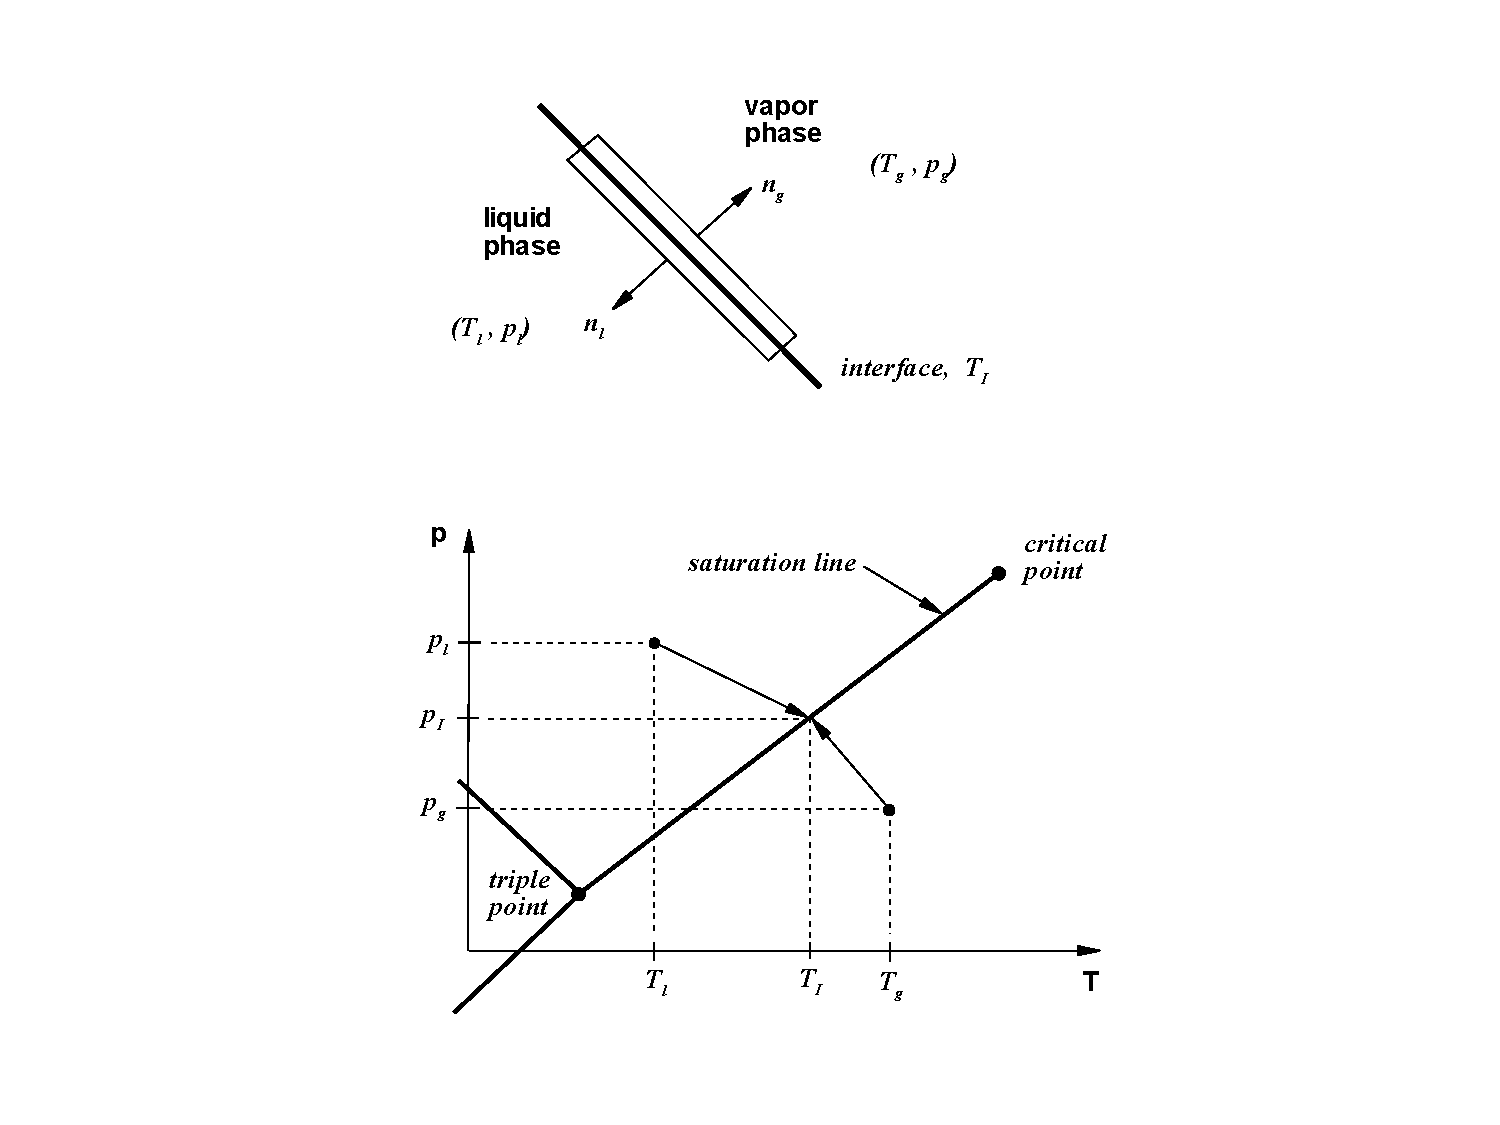
\includegraphics[clip=true,viewport=200 50 550 500,width=.8\textwidth]{figures/saturation}
   % }
   \caption{Interface control volume (top); $T$-$p$ state space around
     saturation line, $T_{liq} < T_{vap}$, (bottom).\label{Berry-Fig:2}}
\end{figure}

To examine the mass flow rate between phases, local mechanisms of the
vaporization (condensation) process are considered between the liquid
phase and its associated vapor in the presence of temperature
gradients.  The mechanisms of interest here are dominated by heat
diffusion at the interface.  The pertinent local equations to consider
are the mass and energy equations.  As a vaporization front propagates
slowly (on the order of 1 mm/s to 1 m/s) compared to acoustic waves
present in the medium (which propagate with speeds of the order 1
km/s), acoustic propagation results in quasi-isobaric pressure
evolution through vaporization fronts.  The momentum equation is
therefore not needed -- because the quasi-isobaric assumption
(neglecting the pressure and kinetic energy variations in the total
energy equation) is made.  A simple expression for the interphase
mass flow rate is obtained
\begin{align}
  \nonumber
  \Gamma = \Gamma_{vap}
  &= \frac{h_{T,  liq} \left( T_{liq} - T_{int} \right) + h_{T,  vap} \left( T_{vap} - T_{int} \right)}{h_{vap,  int} - h_{liq,  int}}
  \\
  &= \frac{h_{T,  liq} \left( T_{liq} - T_{int} \right) + h_{T,  vap} \left( T_{vap} - T_{int} \right)}{L_v \left( T_{int} \right)}
\end{align}
where $L_v \left( T_{int} \right) = h_{vap,  int} - h_{liq,  int}$
represents the latent heat of vaporization.  The interface
temperature is determined by the saturation constraint
$T_{int}=T_{sat}(p)$ with the appropriate pressure $p=\bar{p}_{int}$
determined above, the interphase mass flow rate is thus determined.
The lower graphic of Figure~\ref{Berry-Fig:2}, schematically shows the
$p$-$T$ state space in the vicinity of the saturation line (shown
for the case with $T_{liq} < T_{vap}$).

To better illustrate the model for vaporization or condensation,
Figure~\ref{Berry-Fig:3} shows pure liquid and pure vapor regions
separated by an interface.
\begin{figure}
  \centering
  %\fbox{
   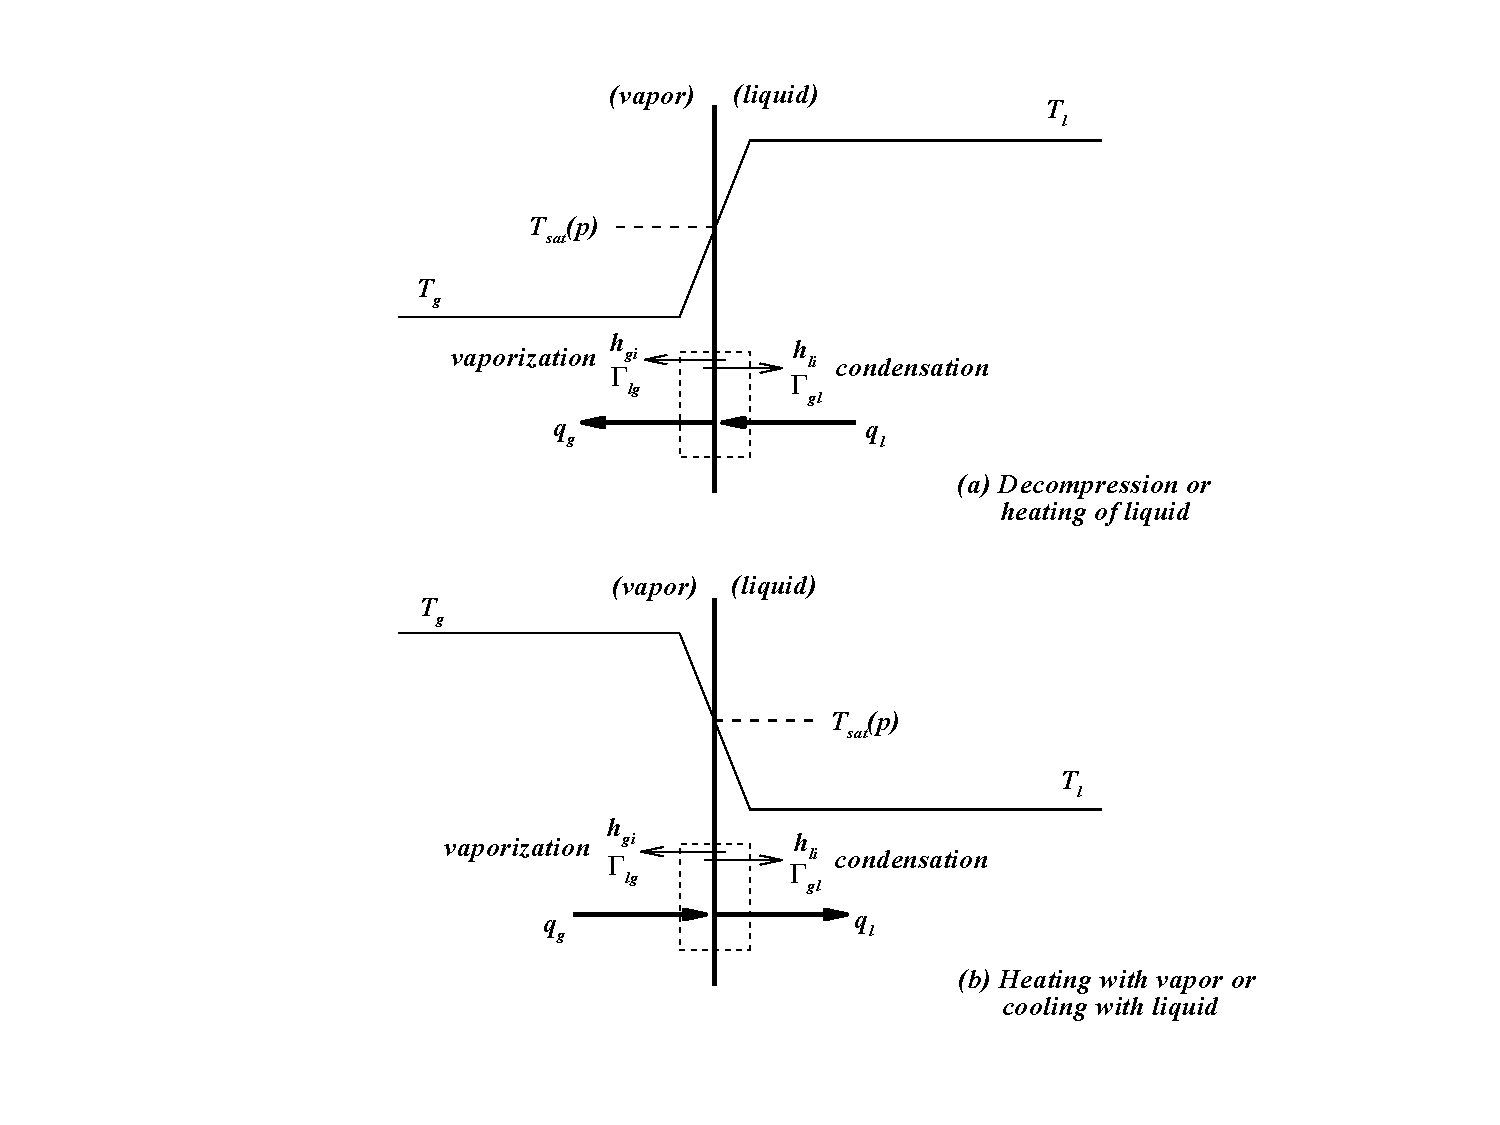
\includegraphics[clip=true,viewport=175 50 625 525,width=.8\textwidth]{figures/vaporization_condensation}
 %}
   \caption{Vaporization and condensation at a liquid-vapor interface
     (after Moody~\cite{Moody_1990}).\label{Berry-Fig:3}}
\end{figure}
Representative temperature profiles are shown for heat transfer from
vapor to liquid or liquid to vapor.  As discussed by
Moody~\cite{Moody_1990}, either vaporization or condensation can occur
for both temperature profiles. The interphase mass transfer is
determined by the net interfacial heat transfer: if net heat transfer
is toward the interface, vapor will form; conversely, if net heat
transfer is away from the interface, liquid will condense.
Figure~\ref{Berry-Fig:3} shows heat transfer rates $q_{vap}$ and
$q_{liq}$ from the vapor and liquid sides of the interface.  For
bidirectional phase change (vaporization and condensation), mass
transfer based on heat balance at the interface is adopted.  When
vaporization occurs, vapor is assumed to form at a saturated interface
temperature $T_{int}=T_{sat}(\bar{p}_{int})$.  If condensation occurs,
liquid is assumed to form also at a saturated interface temperature
$T_{int}=T_{sat}(\bar{p}_{int})$.  The interfacial total enthalpies
correspond to the saturated values in order that the interphase mass
transfer rate and conservation of total energy be compatible:
\begin{equation}
  \label{E-R:95}
  H_{k,  int} = h_{k,  int} + \frac{1}{2} u_{int}^2
\end{equation}
for phase $k=(liq, vap)$, where $h_{k,int}$ is the phase $k$ specific enthalpy
evaluated at the interface condition.  Phasic specific enthalpy
depends upon the equation of state used and will be discussed with the
equations of state.  The interfacial density corresponds to the liquid
saturated density $\rho_{int} = \rho_{liq, sat}(p_{int})$.


\subsubsection{Stiffened Gas Equation of State for Two-phase Flows} \label{sec:SGEOS}
With the 7-equation two-phase model each phase is compressible and
behaves with its own convex equation of state (EOS).  For initial
development purposes it was decided to use a simple form capable of
capturing the essential physics.  For this purpose the stiffened
gas equation of state (SGEOS)~\cite{SGEOS} was selected (as
it was also for single phase)
\begin{equation}
  \label{E-R:96}
  p(\rho,e) = (\gamma -1) \rho (e - q) - \gamma p_{\infty}
\end{equation}
where $p$, $\rho$, $e$, and $q$ are the pressure, density,
internal energy, and the binding energy of the fluid considered.  The
parameters $\gamma$, $q$, and $p_{\infty}$ are the constants
(coefficients) of each fluid.  The first term on the right hand side
is a repulsive effect that is present for any state (gas, liquid, or
solid), and is due to molecular vibrations.  The second term on the
right represents the attractive molecular effect that guarantees the
cohesion of matter in the liquid or solid phases.  The parameters used
in this SGEOS are determined by using a reference curve, usually in
the $\left(p, \frac{1}{\rho}\right)$ plane.

To extend this equation of state for two phases,
LeMetayer~\cite{SGEOS} uses the saturation curves as this
reference curve to determine the stiffened gas parameters for liquid
and vapor phases.  The SGEOS is the simplest prototype that contains
the main physical properties of pure fluids, repulsive and attractive
molecular effects, thereby facilitating the handling of the essential
physics and thermodynamics with a simple analytical formulation.  Thus
each fluid has its own thermodynamics.  For each phase the
thermodynamic state is determined by the SGEOS:
\begin{align}
  \label{E-R:97}
  e(p,\rho) &= \frac{p+\gamma p_{\infty}}{(\gamma -1) \rho} + q
  \\
  \label{E-R:98}
  \rho (p,T) &= \frac{p+p_{\infty}}{(\gamma -1) c_v T}
  \\
  \label{E-R:99}
  h(T) &= \gamma  c_v T + q
  \\
  \label{E-R:100}
  g(p,T) &= \left(\gamma c_v - q'\right) T - c_v T \ln \frac{T^\gamma}{\left(p+p_{\infty}\right)^{\gamma-1}} + q
\end{align}
where $T$, $h$, and $g$ are the temperature, enthalpy,
and Gibbs free enthalpy, respectively, of the phase considered.  In
addition to the three material constants mentioned above, two
additional material constants have been introduced, the constant
volume specific heat $c_v$ and the parameter $q'$.  The method to
determine these parameters in liquid-vapor systems, and in particular
the coupling of liquid and vapor parameters, is given
in~\cite{SGEOS}.  The values for water and its vapor from that
reference are given in Table 2.  These parameter values appear to
yield reasonable approximations over a temperature range from 298 to
473K.  For higher temperature range the parameters can easily be
refit.

Unlike van der Waals type modeling where mass transfer is a
thermodynamic path, with the 7-equation two-phase model the mass
transfer modeling, which produces a relaxation toward thermodynamic
equilibrium, is achieved by a kinetic process.  Thus the 7-equation
model preserves hyperbolicity during mass transfer.
From equation~\eqref{E-R:99} it is readily seen that the phase
$k$ specific enthalpy evaluated at the interface condition from
equation~\eqref{E-R:95} is
\begin{equation}
  h_{k,  int} = c_{p, k}  T_{int} + q_k
\end{equation}
because $c_{p, k} = \gamma_k  c_{v, k}$.

The bulk interphase mass transfer from the liquid phase to the vapor
phase $\Gamma$ is due to their difference in Gibb's free energy.  At
saturated conditions the Gibb's energies of the two-phases are equal.
It is necessary to determine the saturation temperature $T_{sat}(p)$
for given pressure $p=\bar{p}_{int}$ and the heat of vaporization
$L_v\left(T_{sat}(\bar{p}_{int}) \right)$ at this saturation temperature
with the SGEOS for each phase.  For this calculation the procedure
of~\cite{SGEOS} is adopted.  This procedure for the
determination of SGEOS parameters can be made very accurate provided
the two reference states are picked sufficiently close to represent
the experimental saturation curves as locally quasi-linear.
Restrictions occur near the critical point, but away from this point
wide ranges of temperatures and pressures can be considered.  At
thermodynamic equilibrium at the interface, the two phasic Gibbs free
enthalpies must be equal, $g_{vap}=g_{liq}$, so the use of equation~\eqref{E-R:100}
yields
\begin{equation}
  \label{E-R:102}
  \ln \left( p + p_{\infty,  vap} \right) = A + \frac{B}{T} + C  \ln(T) + D  \ln \left( p + p_{\infty,  liq} \right)
\end{equation}
where
\begin{align}
  A &= \frac{c_{p, liq} - c_{p, vap} + q'_{vap} - q'_{liq}}{c_{p,  vap} - c_{v,  vap}} \\
  B &= \frac{q_{liq}-q_{vap}}{c_{p,  vap} - c_{v,  vap}} \\
  C &= \frac{c_{p, vap} - c_{p, liq}}{c_{p,  vap} - c_{v,  vap}} \\
  D &= \frac{c_{p, liq} - c_{v, liq}}{c_{p,  vap} - c_{v,  vap}} \,\,.
\end{align}
Relation~\eqref{E-R:102} is nonlinear, but can used to compute the
theoretical curve $T_{sat}(p)$.  A simple Newton iterative numerical
procedure is used.  With $T_{sat}(p)$ determined, the heat of
vaporization is calculated as
\begin{align}
  \nonumber
  L_v \left( T_{int} \right) &= h_{vap,  int} - h_{liq,  int}
  \\
  \nonumber
  &= h_{k,  int}
  \\
  &= \left( \gamma_{vap}  c_{v, vap}  T + q_{vap} \right) - \left( \gamma_{liq}  c_{v, liq}  T + q_{liq} \right) \,.
\end{align}
%===================================================================================
\section{Derivation of the dissipative terms:}
%===================================================================================
%===================================================================================
\section{The viscosity coefficients:}
%===================================================================================
%===================================================================================
\section{Numerical results:}
%===================================================================================
%\section{This is a Very Long Section Title This is a Very Long Section Title This is a Very Long Section Title }